\documentclass{article}
\usepackage{amsmath}
\usepackage{graphicx}
\usepackage{booktabs}    
\usepackage{array}   
\usepackage{multirow} 
\usepackage{siunitx}

\begin{document}
    \title{Overview of Task 2}
    \maketitle
    In this task, we reconstructed the lower half of each image based on
    the upper half. Specifically, the goal was to predict the missing lower half lever-
    aging information from the upper half, allowing the model to “complete” the
    image of each sign language digit. To achieve this, we experimented with
    various approaches, including ridge regression, principal component regression,
    and kernel ridge regression. Furthermore, we evaluated and compared model
    performance using metrics such as mean squared error (MSE), Structural Simi-
    larity Index Measure (SSIM), and Peak Signal-to-Noise Ratio (PSNR). Finally,
    we explained the differences in model performance and suggested potential ways
    to improve performance.

    \section{Data Preprocessing}
    The analysis began with a data set of images, stored as a NumPy array with shape $(2062, 64, 64)$ (i.e., 2062 images with each image having $64 \times 64$ pixels). First, the original 3D array of shape $(2062, 64, 64)$ was reshaped into a 2D array with shape: $(n, 64 \times 64)$, where each row represents one flattened image. Next, we split the data into 80\% training and 20\% testing sets, and this splitting was performed before separating the upper and lower halves to prevent data leakage. Then, each flattened image is divided at the midpoint for upper-lower-hale separation. The upper half of the images was used as input features, while the lower half of the images was used as target variables.

    \section{Fitting the Three Regression-Based Models for Image Completion}
        \subsection{Ridge Regression (RR)}
        The RR implementation involved standardizing both input features and target variables, followed by ridge regression with cross-validation. The optimization problem for ridge regression is:
        
        \begin{equation}
            \hat{\beta}_{ridge} = \argmin_{\beta} \left\{ \|y - X\beta\|^2 + \alpha\|\beta\|^2 \right\}
        \end{equation}
        
        where:
        \begin{itemize}
            \item $X$ is the standardized input matrix
            \item $y$ is the standardized target vector
            \item $\alpha$ is the regularization parameter, tested for values $\{0.1, 1.0, 10.0, 100.0\}$
            \item $\|\beta\|^2$ is the L2 norm of the coefficient vector
        \end{itemize}
        
        \subsection{Principal Component Regression (PCR)}
        PCR combines PCA with linear regression. The PCA transformation is first computed as:
        
        \begin{equation}
            Z = X W
        \end{equation}
        
        where:
        \begin{itemize}
            \item $W$ is the matrix of eigenvectors of $X^TX$
            \item $Z$ represents the principal components
        \end{itemize}
        
        The first 50 components are retained, and linear regression is performed:
        
        \begin{equation}
            y = Z_{50}\gamma + \epsilon
        \end{equation}
        
        where:
        \begin{itemize}
            \item $Z_{50}$ contains the first 50 principal components
            \item $\gamma$ is the coefficient vector in the transformed space
            \item $\epsilon$ is the error term
        \end{itemize}
        
        \subsection{Kernel Ridge Regression (KRR)}
        KRR extends ridge regression to non-linear patterns using the kernel trick. The optimization problem becomes:
        
        \begin{equation}
            \hat{\alpha} = \argmin_{\alpha} \left\{ \|y - K\alpha\|^2 + \lambda\alpha^T K\alpha \right\}
        \end{equation}
        
        with the RBF kernel function:
        
        \begin{equation}
            K(x_i, x_j) = \exp\left(-\gamma\|x_i - x_j\|^2\right)
        \end{equation}
        
        where:
        \begin{itemize}
            \item $K$ is the kernel matrix with elements $K_{ij} = K(x_i, x_j)$
            \item $\gamma$ is the RBF kernel coefficient
            \item $\lambda$ is the regularization parameter
            \item The prediction for a new point $x_*$ is given by:
            \begin{equation}
                f(x_*) = \sum_{i=1}^n \alpha_i K(x_i, x_*)
            \end{equation}
        \end{itemize}
        
        Hyperparameters were optimized through 5-fold cross-validation:
        \begin{itemize}
            \item Regularization parameter $\lambda \in \{0.001, 0.01, 0.1, 1.0, 10.0\}$
            \item RBF kernel coefficient $\gamma \in \{0.0001, 0.001, 0.01, 0.1, 1.0\}$
        \end{itemize}
    
    \section{Model Evaluation}
    Three different metrics were used to evaluate the quality of the image reconstruction:
    
        \subsection{Mean Squared Error (MSE)}
        MSE measures the average squared difference between predicted and actual pixel values:
            \begin{equation}
                MSE = \frac{1}{n} \sum_{i=1}^{n} (y_i - \hat{y}_i)^2
            \end{equation}
        where $y_i$ represents the true pixel values and $\hat{y}_i$ represents the predicted pixel values.
    
        \subsection{Structural Similarity Index Measure (SSIM)}
        SSIM evaluates the perceived quality between two images $x$ and $y$ by combining three comparative measurements:
        \begin{equation}
            SSIM(x,y) = \frac{(2\mu_x\mu_y + c_1)(2\sigma_{xy} + c_2)}{(\mu_x^2 + \mu_y^2 + c_1)(\sigma_x^2 + \sigma_y^2 + c_2)}
        \end{equation}
        where:
        \begin{itemize}
            \item $\mu_x$, $\mu_y$ are the average pixel values
            \item $\sigma_x^2$, $\sigma_y^2$ are the variances
            \item $\sigma_{xy}$ is the covariance
            \item $c_1$, $c_2$ are constants to avoid division by zero
        \end{itemize}
        SSIM ranges from -1 to 1, with 1 indicating perfect structural similarity.
    
        \subsection{Peak Signal-to-Noise Ratio (PSNR)}
        PSNR measures the ratio between the maximum possible pixel value and the corrupting noise:
        \begin{equation}
            PSNR = 20 \cdot \log_{10}\left(\frac{MAX_I}{\sqrt{MSE}}\right) = 20 \cdot \log_{10}\left(\frac{1}{\sqrt{MSE}}\right)
        \end{equation}
        where $MAX_I$ is the maximum possible pixel value (normalized to 1 in our case). PSNR is expressed in decibels (dB), with higher values indicating better quality reconstruction.
    
        \subsection{Implementation Details}
        For each image in the test set:
        \begin{enumerate}
            \item The lower halves of predicted and true images were reshaped to their original dimensions
            \item SSIM was computed using the maximum pixel range as the data range
            \item PSNR was computed using the MSE of individual images
            \item Final metrics were averaged across all test images:
            \begin{equation}
                \text{Average Metric} = \frac{1}{N}\sum_{i=1}^{N} \text{Metric}_i
            \end{equation}
            where $N$ is the number of test images
        \end{enumerate}
    
        Special consideration was given to the case where MSE = 0 in PSNR calculation, which would result in an infinite value. In such cases, PSNR was set to infinity, indicating perfect reconstruction.

    \section{Results and Discussion}
        Table \ref{table:model_comparison} below outlines the performance of the three models for the image completion task. The comparative analysis of the three regression methods reveals a clear performance hierarchy in the image completion task. Kernel Ridge Regression (KRR) demonstrated the best overall performance with the lowest MSE (0.0123), highest SSIM (0.4425), and highest PSNR (19.4289 dB), likely due to its ability to capture non-linear relationships through the RBF kernel. Principal Component Regression (PCR) showed intermediate performance (MSE: 0.0131, SSIM: 0.4251, PSNR: 19.0970), suggesting that dimensionality reduction to 50 principal components preserved significant image features while reducing noise. Ridge Regression (RR) exhibited the least favorable performance (MSE: 0.0153, SSIM: 0.4045, PSNR: 18.5663), indicating that linear relationships alone were insufficient for this complex image completion task. However, the moderate SSIM values (below 0.5) across all models suggest that there is still room for improvement, possibly through more advanced techniques such as deep learning approaches.
        \begin{table}[h]
            \centering
            \caption{Performance Comparison of Different Regression Methods}
            \begin{tabular}{l
                            S[table-format=1.4]
                            S[table-format=1.4]
                            S[table-format=2.2]}
            \toprule
            {Method} & {MSE} & {SSIM} & {PSNR} \\
            \midrule
            RR & 0.0153 & 0.4045 & 18.5663 \\
            PCR & 0.0131 & 0.4251 & 19.0970 \\
            KRR & 0.0123 & 0.4425 & 19.4289 \\
            \bottomrule
            \end{tabular}
        \label{table:model_comparison}
        \end{table}

        Meanwhile, Figure \ref{fig:completion_comparison} presents a visual comparison of image completion results across five different hand gestures, comparing the original images with reconstructions from RR, PCR, and KRR methods. All three methods successfully capture the general hand structure and finger positions, but differ in their reconstruction quality of fine details and background transitions. RR, while capturing the basic hand shape, shows the most noticeable artifacts and less smooth transitions, particularly visible in the background regions and along the finger edges. KRR demonstrates the most faithful reconstruction, particularly in preserving the smooth transitions between the hand and background, and maintaining consistent color gradients. PCR shows comparable performance to KRR in maintaining the overall hand structure but exhibits slightly more artifacts in the background regions. These visual results align with the quantitative metrics, confirming KRR's superior performance in maintaining both structural integrity and detail preservation. 
        \begin{figure}[H]
            \centering
            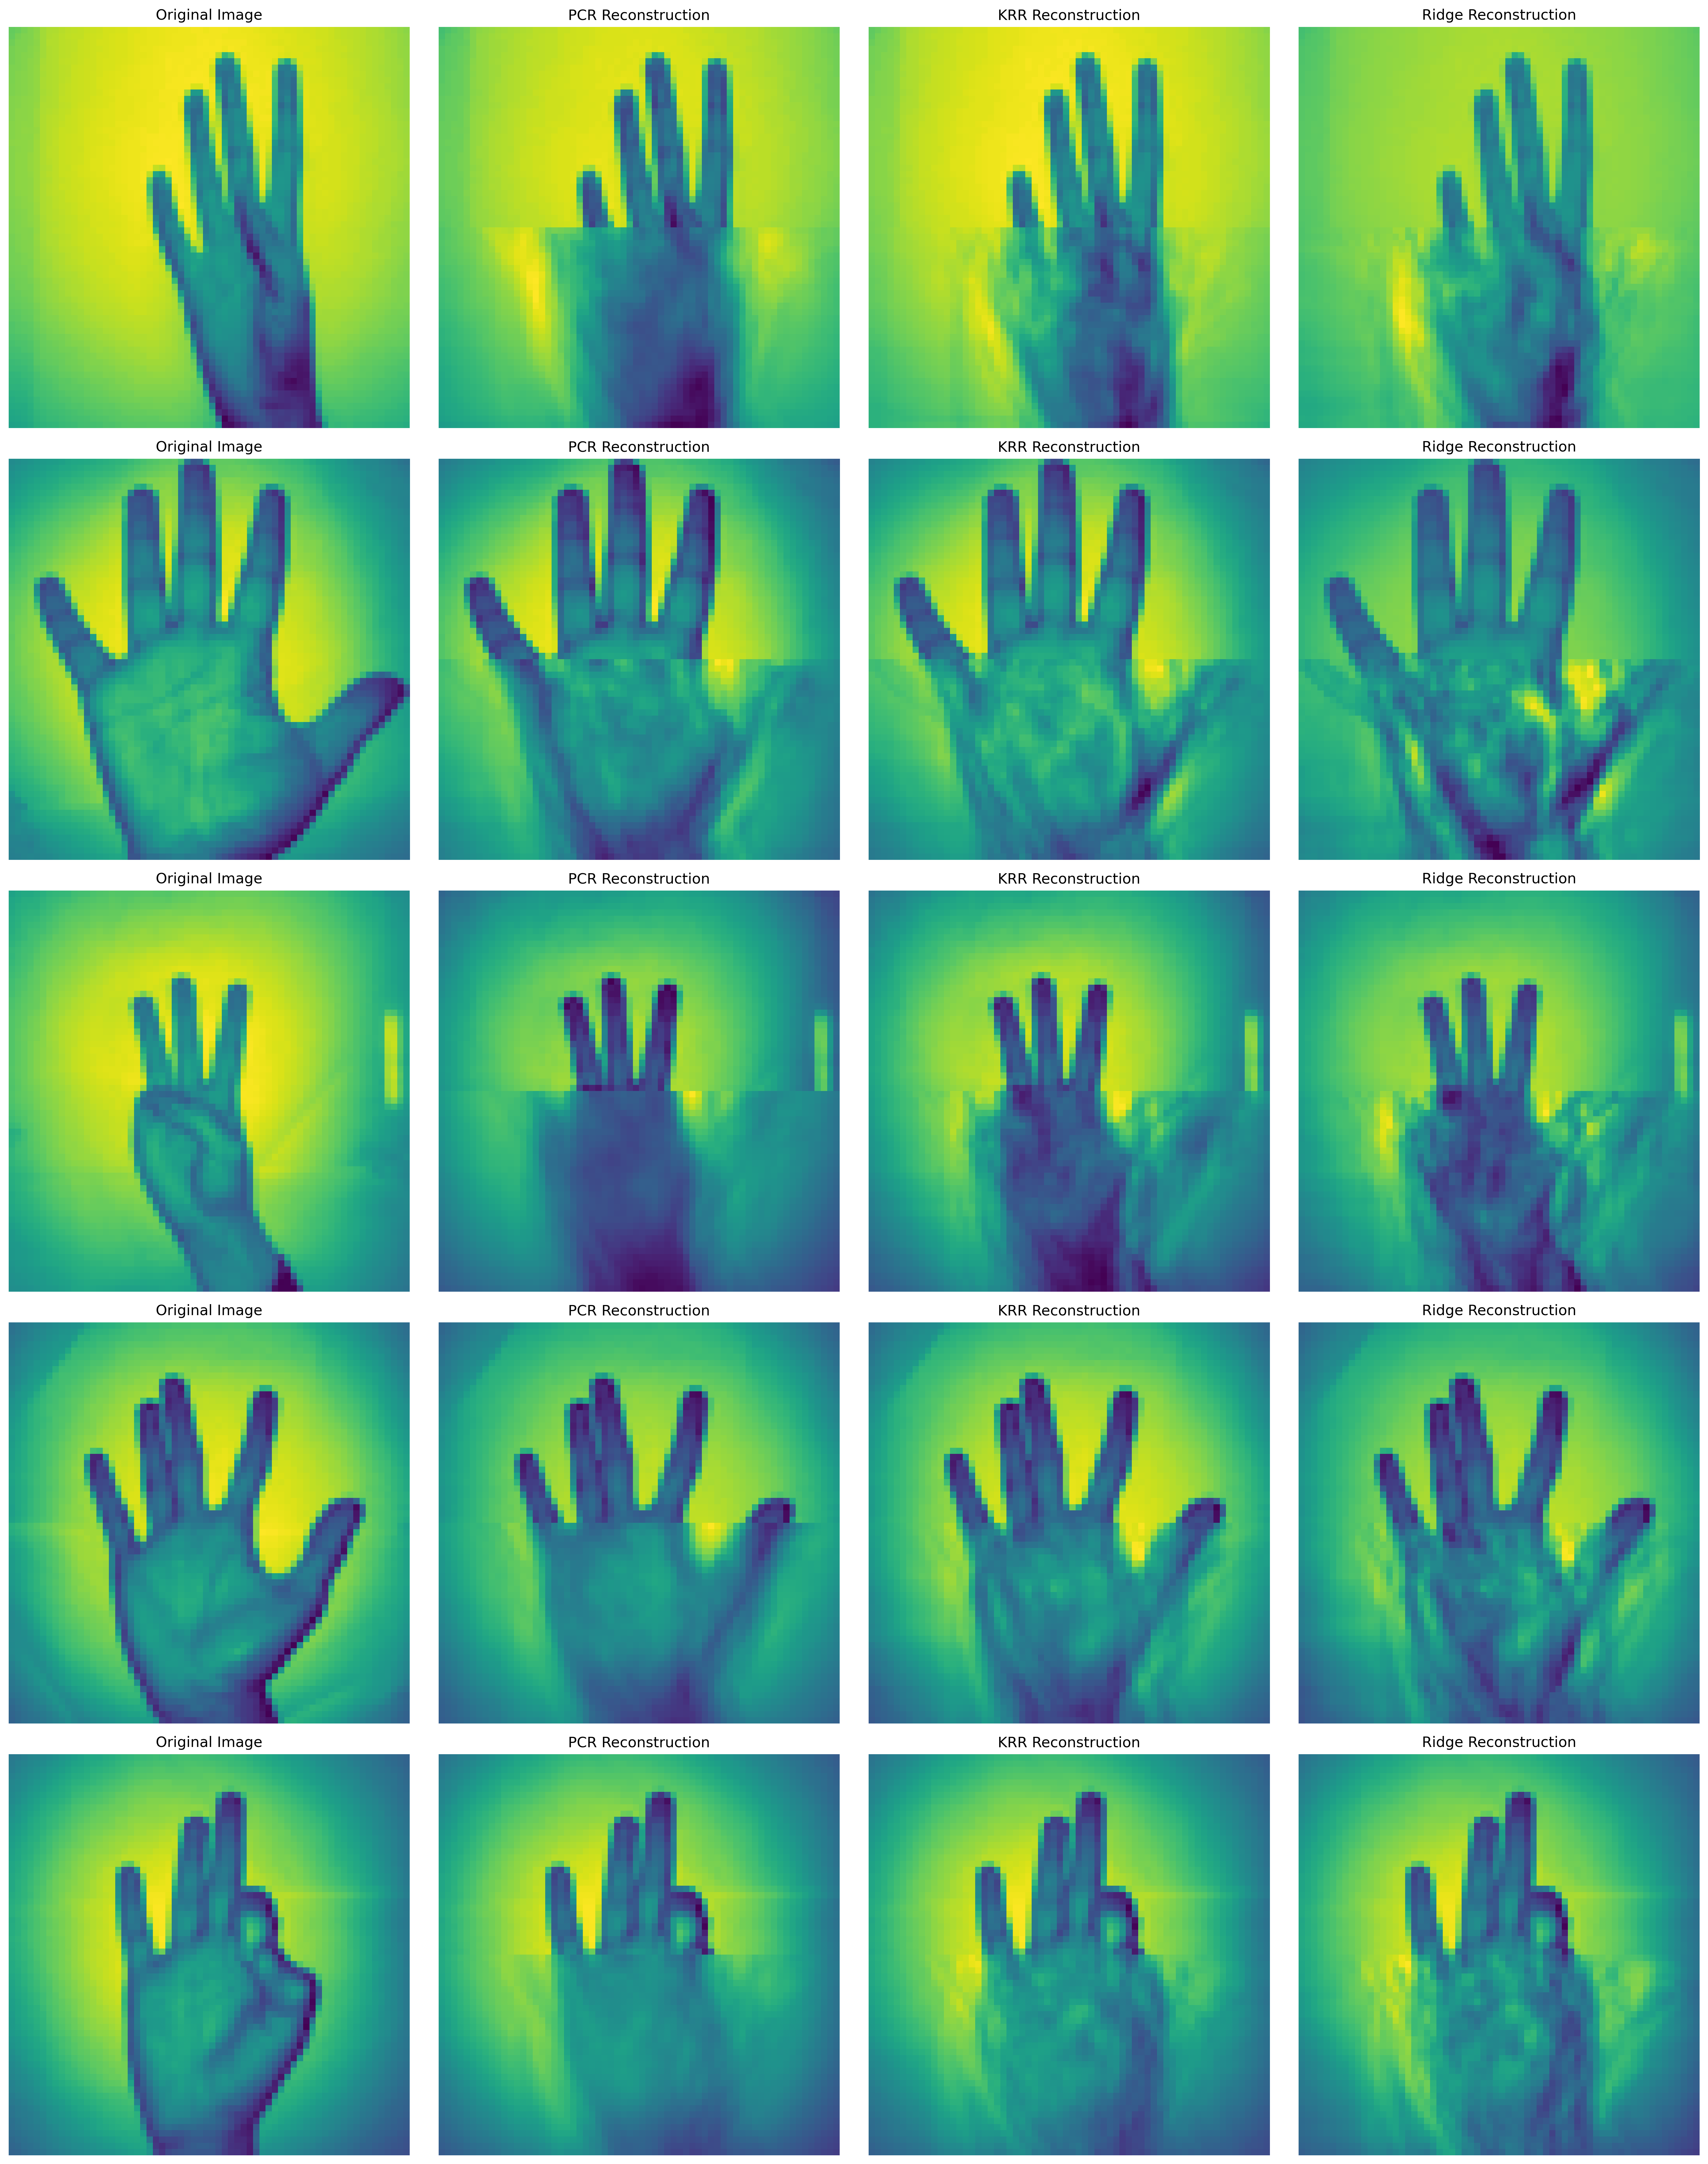
\includegraphics[width=\textwidth]{image_completion_comparison.png}
            \caption{Comparison of image completion results using different regression methods. From left to right: Original image, PCR reconstruction, KRR reconstruction, and Ridge reconstruction.}
            \label{fig:completion_comparison}
        \end{figure}

    The comparative analysis of the three regression methods reveals distinct performance patterns, with KRR demonstrating superior results due to its ability to capture non-linear relationships through the RBF kernel, while PCR's moderate performance with 50 principal components suggests effective dimensionality reduction, and Ridge Regression's basic performance highlights the limitations of linear approaches in complex image completion tasks. Looking forward, several promising avenues for improvement exist, including the implementation of advanced neural network architectures such as Convolutional Autoencoders, U-Net, and GANs, enhancement of feature engineering through edge detection and wavelet transforms, and model refinements via ensemble methods and alternative kernel functions. These potential improvements, particularly the deep learning approaches, could address the current limitations in capturing complex image patterns and potentially yield more sophisticated reconstruction results.
    
\end{document}
